\exer{[pont-de-wheatstone]}
\setcounter{numques}{0}~\\

\question{} Calculer la valeur de l'intensité $i$ dans les deux cas suivants :
		\begin{enumerate}
			\item $E = 10$ V ; $R_1 = R_3 = 10 \text{ k} \Omega$ ; $R_2 = R_4 = R = 1 \text{ k} \Omega$ ;
			\item $E = 10$ V ; $R_1 = R_3 = 4 \text{ k} \Omega$ ; $R_2 = R = 2 \text{ k} \Omega$ ; $R_4= 8 \text{ k} \Omega$.
		\end{enumerate}

		\begin{enumerate}
			\item
\begin{xxpyconsole}%~\\ \vspace{-.5cm}
\begin{pyconsole}
import numpy as np
import matplotlib.pyplot as plt


R1,R3,R2,R4,R=10**4,10**4,10**3,10**3,10**3
E=10
A=np.array([[1,-1,0,0,-1],[0,0,1,-1,-1],[R1,R2,0,0,0],[0,0,R3,R4,0],[R1,0,0,-R4,R]])
B=np.array([[0],[0],[E],[E],[0]])
Xa=np.linalg.solve(A,B)
print(Xa)
\end{pyconsole}
\end{xxpyconsole}
			\item
\begin{xxpyconsole}%~\\ \vspace{-.5cm}
\begin{pyconsole}
import numpy as np
import matplotlib.pyplot as plt


R1,R3,R2,R4,R=4*1e3,4*1e3,2*1e3,8*1e3,2*1e3
E=10
A=np.array([[1,-1,0,0,-1],[0,0,1,-1,-1],[R1,R2,0,0,0],[0,0,R3,R4,0],[R1,0,0,-R4,R]])
B=np.array([[0],[0],[E],[E],[0]])
Xb=np.linalg.solve(A,B)
print(Xb)
\end{pyconsole}
\end{xxpyconsole}
\end{enumerate}

\question{} Le second cas correspond au cas d'un point \textit{équilibré.} En observant la valeur de $i$ trouvée en déduire une relation entre les résistances $R_1$, $R_3$, $R_2$ et $R_4$.



Dans le second cas, le pont de Wheatstone est dit \textit{équilibré}. L'intensité $i$ est nulle et cela correspond à l'égalité :
\[ R_1\times R_3=R_2\times R_4. \]


\question{} Après avoir importé le module \texttt{random}. \'{E}crire un programme permettant :

				\begin{enumerate}
				\item de résoudre le système pour des valeurs de $R_3$ comprises entre $1\text{ k} \Omega$ et $20\text{ k} \Omega$ (on prendra $100$ valeurs) ;
				\item d'afficher la courbe de l'intensité $i$ en fonction de la résistance $R_3$.
				\end{enumerate}
				
\begin{lstlisting}
R1,R4,R=10**3,2*10**3,10**3
R2=(random.randrange(11)+5)*500
E=10

t=np.linspace(10**3,2*10**4,100) # valeurs de R3
i=[]
for R3 in t:
    A=np.array([[1,-1,0,0,-1],[0,0,1,-1,-1],[R1,R2,0,0,0],[0,0,R3,R4,0],[R1,0,0,-R4,R]])
    B=np.array([[0],[0],[E],[E],[0]])
    X=np.linalg.solve(A,B)
    i=i+[X[4,0]*1000] # *1000 pour recuperer une intensite en mA
plt.plot(t,i)
plt.axhline()
plt.savefig('tp13_durif_q7.png')
\end{lstlisting}

\question{} \`{A} l'aide d'une lecture graphique, en déduire la valeur de la résistance $R_2$.

\begin{center}
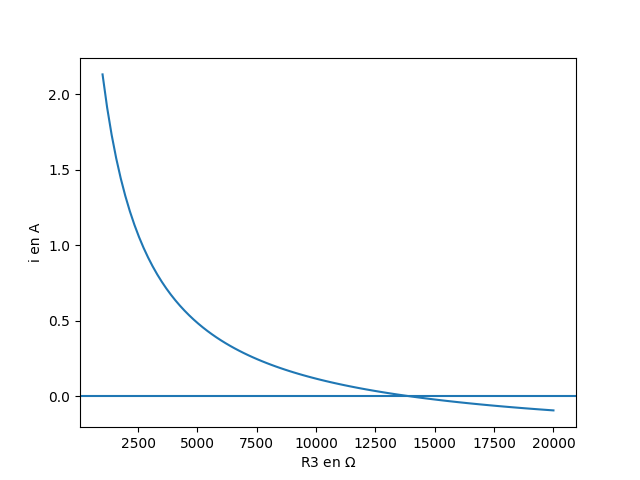
\includegraphics[width=0.5\textwidth]{tp13_durif_q7.png}
\end{center}


